\documentclass[11pt]{article}
\usepackage{geometry} % see geometry.pdf on how to lay out the page. There's lots.
\usepackage{hyperref}
\usepackage{graphicx}
\usepackage{gensymb}
\usepackage[affil-it]{authblk}
\usepackage[toc,page]{appendix}
\usepackage{pifont}
\usepackage{amsmath}
\usepackage{amsthm}

\usepackage{float}

\newtheorem{theorem}{Theorem}
\newtheorem{corollary}{Corollary}
\newtheorem{conjecture}{Conjecture}
\newtheorem{proofsketch}{Proof Sketech}
\usepackage{draftwatermark}

\SetWatermarkText{DRAFT}
\SetWatermarkScale{6}
\SetWatermarkLightness{0.95}

% \geometry{letter} % or letter or a5paper or ... etc
% \geometry{landscape} % rotated page geometry

% See the ``Article customise'' template for come common customisations

\title{A Continuum of Member-length Optimal Untwisted Boerdijk--Coxeter Helices (v0.3)}
\author{Robert L. Read
  \thanks{read.robert@gmail.com}
}
\affil{Founder, Public Invention, an educational non-profit.}


\date{\today}

%%% BEGIN DOCUMENT
\begin{document}

\maketitle

%% \tableofcontents

\begin{abstract}
  The Boerdijk--Coxeter helix (BC helix, or tetrahelix) is a face-to-face stack of regular tetrahedra whose outer vertices lie on helices.
  By allowing changes to edge lengths so that the tetrahedra are not regular, we can define a continum of tetrahelices isomorphic to the
  BC helix of designable pitch or curvature, effectively ``untwisting'' the BC helix. We show that in the sense of minimal maximum
  difference in edge length, every tetrahelix has vertices equally spaced along the axis and at most three distinct edge lengths.
  In the case of a full untwisting to zero curvature, we describe a novel object, the
  \emph{equitetrabeam}.
  It has 3-fold symmetry about  axis, and chirality.  This tetrabeam and controllably twisted tetrahelices are
  interesting for structural engineering because they are inherently rigid space frames and trusses.
  A formula for the cartesian coordinates of the individual nodes of outer helices of the BC helix is given and
  unified with the formula for the equitetrabeam creating a class of edge-length optimal tetrahelices generated by single parameter.
  A further generalization is provided.
  Utility and use for truss/space frame design and robotics are discussed.
\end{abstract}


\section{Introduction}

The Boerdijk--Coxeter helix\cite{coxeter1985simplicial} (BC helix),
is a face-to-face stack of tetrahedra that winds about a straight axis.
The vertices of the tetrahedra
lie upon three
helices about the central axis.
The Tetrobot/Glussbot\cite{TetrobotBook} project
uses the regularity of this geometry to make a tentacle-like robot that can crawl like a slug or mollusc.
The Tetrobot concept
is to use mechanical members, called actuators, which can change their length, connected by special joints, called the Song-Kwon-Kim\cite{song2003spherical} or turret joint,
which allow many
members to come to a single point.
Such machines can follow purely regual mathematical models such as the Boerdijk–-Coxeter helix or the Octet Truss\cite{richard1961synergetic}.
Because architects, structural engineers, and robotocists are inspired by and follow such mathematical models but can build
structures and machines of differing or even dynamically changing length, it is useful to develop
the mathematics of structure formed from tetrahedra where we relax regularity. Buckminster Fuller called the BC helix a \emph{tetrahelix}\cite{fuller1982synergetics},
a term now commonly used. In this paper we reserve BC helix to mean the purely regular structre and use \emph{tetrahelix} to refer
to any structure isomophic to a the BC helix, whether regular or not.

\begin{figure}[H] %float with two figures
  \centering
     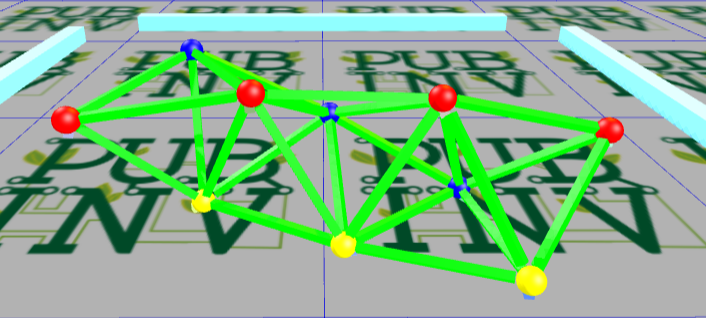
\includegraphics[width=0.4\textwidth]{figures/Tetrahelix0.png}
     \caption{Regular Tetrahelix}
\end{figure}

BC helix does not rest on a plane in a simple way. It is convenient to be able to ``untwist'' it and form a tetrahelix space frame that
has a flat planar surface. By making length changes in a certain way, we can untwist a tetrahelix to form a \emph{tetrabeam} which
has planar faces and has, for example, an equilateral triangular profile.

\section{A User's Formulation of the BC Helix}

If you can choose member lengths, you can form a linear combination of the equitetrabream lengths and the completely regular
lengths of the tetrahelix, thereby choosing the torsion.  If you are designing a space frame, this is a static design choice,
in a robot, it is a dynamic choice that can be used to twist the robot and/or exert torsion on the environment.

Ideally we would have a simple formula for defining the nodes based on any torsion we choose.
Unfortunately, it is not obvious that a linear combination of lengths produces a simple formula.
It is a goal of this paper to relate these two approaches to generating a tetrahelix continuum.

Coxeter constructs the BC helix\cite{coxeter1985simplicial} as a repeated rotation and translation of the tetrahedra, showing the
rotation is:
\[
\theta = \arccos(-2/3) 
\]
and the translation:
\[
h_{bc} = 1/\sqrt{10}
\]


$\theta$ is approximately $131.8103149$ degrees.
The angle $\theta$ is the rotation of a \emph{each} tetrahedra.
That is, a yellow tetrahedron is rotated slightly more than a $1/3$ of a revolution to match the face of the red tetrahedra.
$3 \theta - 2\pi$ is the apparent rotation of $V_3$ relative to $V_0$.

From Robert Gray's site, repeating formula by H.S.M. Coxeter:
\[
V(n) =
\left [
  \begin{tabular}{c}
   $ r_{bc} \cos(n \theta $\\
   $ r_{bc} \sin(n \theta) $\\
   $ n h_{bc}  $
  \end{tabular}
  \right ],
\text{where:}
  \begin{tabular}{c}
 $ r_{bc} = \frac{3\sqrt{3}}{10} $\\
 $ h_{bc} = 1/\sqrt{10} $ \\
 $ \theta = \arccos(-2/3) $ \\
  \end{tabular}      
\]
where $n$ represents each integer numbered node in succession.

This formula defines a helix, but it is not any of the helices of the BC helix, but rather one that winds three times
as rapidly through all nodes. To a designer of tetrahelices, it is more natural to think of the three helices which
are visually apparent, that is, those three which are closely approximated by the by the outer edges or rails of the BC helix.

It is convenient to have a formula that gives us the nodes of just
each colored helix.
\[
H_{BCcolored}(n,c) = V(3n +c)
\]
where $c \in \{0,1,2\}$ specifies which of the rails is being computed.

Such a helix can be written:
\[
H_{BCcolored}(n,c) =
\left [
  \begin{tabular}{c}
   $ r_{bc}  \cos((3 \theta - 2 \pi)n + c  \theta $\\
   $ r_{bc} \sin((3 \theta - 2 \pi)n + c  \theta $\\
   $ (n + c/3) 3  h_{bc} $
  \end{tabular}
  \right ],
\text{where:}
  \begin{tabular}{c}
 $ r_{bc} = \frac{3\sqrt{3}}{10} $\\
 $ h_{bc} = 1/\sqrt{10} $ \\
 $ \theta = \arccos(-2/3) $ \\
  \end{tabular}      
  \]

In this formula, integral values of $n$ may be taken as a node number for one rail and used to compute its Cartesian
coordinates. Allowing $n$ to take non-integer values defines a continuous
helix in space which is close to the segmented polyline of the outer tetrahedra edges, and coincides with them at integer
values.
The parameter $c \in \{0,1,2\}$ specifies which of the rails is being computed.

The quantity $ (3 \theta - 2 \pi) \approx 35.43 \degree $, and is the angular shift between $V(n,color)$ and
$V(n+1,color)$. This quantity appears so often below that we call it the ``rail angle rho'', $\rho_{bc} = (3 \theta - 2 \pi)$.

\begin{figure}[H]
  \label{railanglefig}
     \centering
     \includegraphics[width=0.7\textwidth]{figures/RailAngleGeometry.png}
     \caption{Rail Angle Geometry}
 \end{figure}

Since:
\[ \frac{2 \pi}{\rho_{bc}} \approx 10.16
\]
We can see that there are approximately $10.16$ red, blue or yellow tetrahedra on one rail in a single revolution.
The pitch of the Boerdijk--Coxeter helix of edge length $1$ is the length of three tetrahedra times this number:
\begin{align*}
  &= \frac{3 \cdot h_{bc} 2 \pi }{\rho_{bc}} \\
  &= \frac{3  \sqrt{\frac{2}{5}}  \pi}{\rho_{bc}} \\
  &\approx 9.6392 \\
\end{align*}
The pitch is less than the number of tetrahedra because the tetrahedra are not lined up perfectly.
It is a famous and interesting result that the pitch is irrational, a BC helix never has two tetrahedra
at precisely the same orientation around the $z$-axis. However, this is inconvenient to designers, who
might prefer a rational pitch. For example, a slight irregularity that led to a pitch of precisely 10 tetrahedra
in one revolution would allow an architect to design a column that a basis and a capital in the same relation to the tetrahedra
they touch.
We later provide a means of obtaining that more general tetrahelices.

A BC helix has the useful property that every member is precisely the same length. If we relax this, so that the tetrahedra it
comprises are not perfectly regular, then we can twist and curve the tetrahelix into a variety of shapes. This is useful to
the mechanical engineer or robotocist because the structure remains an inherently rigid, omni-triangulated space frame, which
may be expected to be at least somewhat mechanically strong.

In particular, by designing by hand, much as a sculptor might, we can the lengths of individual members of the BC helix to reduce the
twist or even form a tetrabeam.
However, we seek an algorithm or formula for a tetrabeam that is irregular
(in terms of its tetrahedra) but as regular as possible in terms of mechanical engineering to be comprehensible and computationally tractable.
Observe that a regular BC helix appears to have three bumpy ``rails'' which wind about the central axis.  We seek to untwist
these rails so they form a track is a plane.

In order to do this for an tetrahelix of arbitrary length, we need a naming convention for each member. We propose a coloring
scheme in which the joints and members on the outer ``rails'' of the tetrahelix are colored in primary colors red, yellow and blue.
We propose that the interior members be colored based on the rails they connect using an subtractive color scheme, or orange, purple, and green,
if the member connects red to yellow, red to blue, or blue to yellow, respectively.  Furthermore, we call interior members ``even'' if they
are even numbered starting from the joint at the origin, and ``odd'' if they are odd-numbered.  We have found that nine classes thus
formed are sufficient to untwist the tetrahelix and for our purposes: $red, yellow, orange_{even}, orange_o, purple_e, purple_o, green_e, green_o$.
In the diagram below, the ``odd'' members are draw with a dashed line.


 \begin{figure}[H]
     \centering
     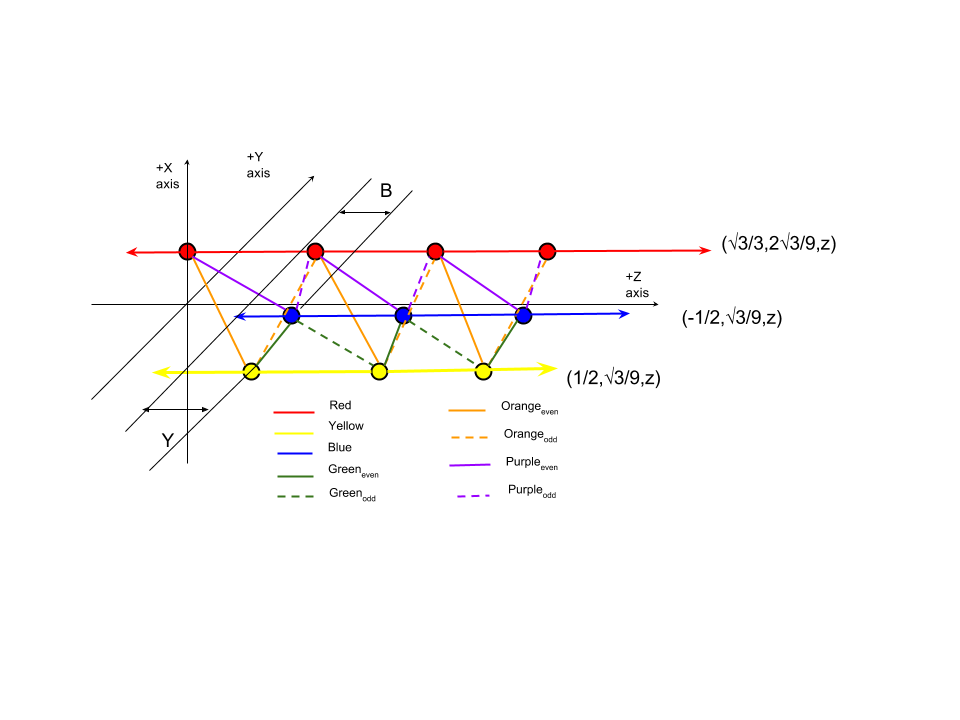
\includegraphics[width=0.9\textwidth]{figures/TetrahelixColoringDiagram.png}
     \caption{Coloring of an (untwisted) Tetrabeam}
 \end{figure}


  That is, in our coloring scheme, $V_0$ is red, and$ V_1$ is yellow,  $V_2$ is blue,
  $V_3$ is red, etc.

\begin{theorem}
  Suppose that all edges are on a cylinder and that $R,B,Y$ are on lines $120\degree$ from each other.
  Then at minimax positioning occurs when at least 3 non-rail edge classes are the longest length and equivalent.
 \end{theorem}
\begin{proof}
  Suppose that all edges are on a cylinder and that $R,B,Y$ are on lines $120\degree$ from each other. Observe
  that the distance between any two nodes of different color is at least $1$, and between the same colors (``on the same rail'') exactly $1$ if closest.

  If there is a unique longest distance, it touches two rails. Moving those rails closer together infinitesimally decreases the longest length and
  therefore the minimax.

  Suppose there are exactly two longest edges of equal length. By the pigeonhole principle, these edges must share one rail and touch the other two.
  If moving the shared rail in one direction decreases both edge lengths, doing so infinitesimally decreases the minimax.

  Therefore there must be at least three longest edges of equal length, each of which touches two rails.
  \end{proof}

\begin{theorem}
  Any minimax-optimal tetrahelix at most precisely three classes of edge lengths.
\end{theorem}

\begin{proof}
  Every vertex is connected to each rail by two edges. These two edges cannot be of the same length, unless all six edge classes are the same
  length. If all six are the same length, $Y_0$ and $B_0$ lie on the same $z$ value, but then $green_o$ is much longer than $purple_e = purple_o = orange_e = organge_o$,
  making it a unique longest length, a contradiciton. Therefore the odd and even lengths in each color class are different. Therfore there is a second,
  shorter length, which occurs once in each color class. Taken with the rail edge length of $1$, this makes precisely three classes of equivalent
  edge lengths for any minimax-optimal helix.
\end{proof}
  
\begin{theorem}
  \label{tetrahelixoptimality}
  Any one tetrahedron in a minimax-optimal tetrahelix $ABCD$ of edge lengths $AD = 1, AB = BC = CD = u , AC = BD = v$, where $1 \leq u \leq v$.
  Any one tetrahedron in a tetrahelix has $1$ rail edge, $2$ mid-length edges connected to the rail and $2$ long edges connected to the rail.
  The edge opposite of the rail edge is a mid-length edge.
\end{theorem}

\begin{proof}
The edge opposite of the rail edge is a mid-length edge because between any two rails the edges alteranate mid-length and long.
\end{proof}

\begin{corollary}
  \label{eventhirds}
  Any minimax optimal tetrahelix has its colored edges spaced at 1/3 the height of
  a tetrahedra along the z-axis, where the height is the z-distance of the rail edge.
  \end{corollary}

\begin{proof}
  Let the variables $O,G,P$ represent the z-axis distance from the
  $R_0$ to $Y_0$, $Y_0$ to $B_0$, and
  $B_0$ to $R_0$ respectively. Then $O+G+P = h$. But $O=G=P$, since each edge between
  their nodes spans two rails of the same distance with an edge of the same length,
  so that the $z$-distance between each node is the same. So $O=G=P=h/3$.
\end{proof}

Note that based on Theorems \ref{tetrahelixoptimality} and \ref{eventhirds}, we are justified in classifying edge lengths as \emph{rail},\emph{mid-length}, or
\emph{long}. The mid-length edges are the edges between closest on the $z$-axis, and the long edges are those that hop over a vertex.

Every optimal tetrahelix has vertices lying on helices expressible in the form:
\[
V_{optimal}(n,c) =
\left [
  \begin{tabular}{c}
   $ r \cos(n \alpha +  c 2 \pi /3)$\\
   $ r \sin(n \alpha +  c 2 \pi /3) $\\
   $ \frac{d(n +c / 3)}{3}   $
  \end{tabular}
\right ]
\]
where we have not yet investigated in the general case the relationships beteween $\alpha$, $r$, and $d$ in this formulation.
However, we understand that when $\alpha = 0$, the helices are degenerate, having curvature of $0$, and
we have the equitetrabeam.






\section{Adding an Untwisting Parameter}

We observe that it by thinking of the straight lines of the Equitetrabeam as a degenerate helix of zero curvature,
it should be possible to define a smoothly varying continuum between the Boerdijk--Coxeter helix and the Equitetrabeam and every
curvature and torsion between the two.

This formulation $V(n,c)$ above is valuable, but obscures the essentially fact that the red, yellow, and blue helices distributed
about the central $z$ axis $120\degree$ from each other.
In order to rewrite this expression with an explicit rotation of $2\pi/3$, we expand 
the expression and seek to isolate the term $c2\pi/3$.
\begin{align*}
  \rho_{bc} n + c \theta  &=   \text{\{we aim for 3 in denominator, so we split...\}} \\
    (3 \theta - 2 \pi)n + (c/3)  (\theta /3)  &=   \text{\{we want $2\pi$ in numerator, so add canceling terms...\}} \\
  (3 \theta - 2 \pi)n + (c/ 3) (3 \theta - 2 \pi  + 2 \pi) &=  \text{\{associate...\}} \\
  (3 \theta - 2 \pi)n + (c/ 3) ((3 \theta - 2 \pi)  + 2 \pi) &=  \text{\{distribute...\}} \\  
  (3 \theta - 2 \pi)n + (c / 3) (3 \theta - 2 \pi)  + c 2 \pi /3 &=  \text{\{definition of $\rho_{bc}$...\}} \\
  \rho_{bc} n + (c / 3) \rho_{bc}  + c 2 \pi /3 &=  \text{\{collect like factors...\}} \\  
  \rho_{bc} (n + c/3)  + c 2 \pi /3  \\
\end{align*}
Now the the term on the left is the only one that depends on the scalar $n$. We use this to a create
a new formulation $H_{BCsymmetric}(n,c) = H_{colored}(n,c)$

The expression $n+c/3$ will now occur so often that we call it the ``c($\kappa$)olored number'' and we use the variable $\kappa$ to represent it: $\kappa = n+c/3$.
Recall that $c \in \{0,1,2\}$, but $n$ and $\kappa$ are are continuous (rational or real-valued.)

\[
H_{BCsymmmetric}(n,c) =
\left [
  \begin{tabular}{c}
   $ r  \cos(\rho_{bc} \kappa  + c 2 \pi /3) $\\
   $ r  \sin(\rho_{bc} \kappa  + c 2 \pi /3) $\\
   $ \kappa 3  d $
  \end{tabular}
  \right ],
\text{where:}
  \begin{tabular}{c}
 $\kappa = n + c/3$ \\
    $\rho_{bc} = (3 \theta - 2 \pi)$ \\
   $ \theta = \arccos(-2/3) $
  \end{tabular}      
\]

We seek to unify this with degenerate helix formula for the equitetrabeam:
\[
H_{etb}(n,c) =
\left [
  \begin{tabular}{c}
   $ r_{etb}  \cos( 0 \cdot \kappa  + c 2 \pi /3) $\\
   $ r_{etb}  \sin( 0 \cdot \kappa  + c 2 \pi /3) $\\
   $ \kappa d_{etb} $
  \end{tabular}
\right ],
\text{where:}
  \begin{tabular}{c}
 $\kappa = n + c/3$ \\
    $\rho_{bc} = (3 \theta - 2 \pi)$ \\
   $ \theta = \arccos(-2/3) $
  \end{tabular}      
\]
where $ r_{etb} = 1/\sqrt(3)$, $d_{etb} = 1/3$,

Now basic components of the helix, which are the radius $r$, the rate of rotation, and the rate of
axial growth can all be linearly interpolated with a parameter $\lambda$ between their high values (for the BC helix)
and low values (for the equitetrabeam):

\begin{align*}
r_{\lambda}  &=  \lambda (3 \sqrt(3) / 10 - 1/\sqrt(3)) +  1/\sqrt(3) \\
d_{\lambda} &=   \lambda (3 / \sqrt(10) - 1)+ 1 \\
\phi_{\lambda} &=  \lambda \rho_{bc}  + 0\\
\end{align*}
to create a formula that generates a continuum of tetrahedral structures:

\[
H_{continuum}(n,c,\lambda) =
\left [
  \begin{tabular}{c}
   $ r_{\lambda} \cos(\phi_{\lambda} \kappa + c 2 \pi /3) $\\
   $ r_{\lambda}  \sin(\phi_{\lambda} \kappa + c 2 \pi /3) $\\
   $ d_{\lambda} \kappa $
  \end{tabular}
  \right ],
\text{where:}
  \begin{tabular}{c}
    $\kappa = n + c/3$ \\
    $ \phi_{\lambda} =  \lambda \rho_{bc}  + 0 $\\
    $\rho_{bc} = (3 \theta - 2 \pi)$ \\
   $ \theta = \arccos(-2/3) $
  \end{tabular}      
\]
A value of $\lambda = 0$ generates the equitetrabeam, and $\lambda = 1$ generates the Boerdijk--Coxeter helix, and every
value $\lambda \in [0,1]$ generates an attractive structure which if physically realized is an inherently rigid structure
with member lengths of no greater disparity than $21\%$.
In the sense of structural engineering, it would be a relatively strong space frame.

Furthermore, this formula allows one to design the pitch (in edge length units) as a function of $\lambda$ of the helix (along one rail)
where $\lambda \neq 0$:
\[
p(\lambda) = 2 \pi  \cdot \frac{((3/\sqrt(10) -1) \lambda +1)}{ \lambda  \rho_{bc} }
\]

\section{Parametrizing Tetrahelices via Rail Angle}

Although the $\lambda$ parametrization presented above is a sensible one
because it unifies the BC-helix with the equitetrabeam, it is over-specific,
in that it makes a specific choice as to the relationship of the height $h$
to the radius $r$ which is somewhat arbitrary.

We seek a formula to generate optimal tetrahelices that accepts a
parameter that allows us to choose the tetrahelix conveniently. The
pitch of the helix is an obious choice, but is not defined when the
curvature is $0$, and important special case. The radius or the axial
distance between two nodes on the same rail are obvious choices, but
perhaps the clearest choice is to build formula that takes as its
input the ``rail angle'' $\rho$. We define $\rho$ to be the angle
formed in the X,Y plane $\angle R_i O R_{i+1}$ projecting out the $z$
axis and sighting along the positive $z$ axis. In other words, $\rho$
controls how far a rail edge of a tetrahelix deviates from being
parallel with the axis, or the ``twistiness'' of tetrahelix. Ideally
we will treat a positive angle as creating a clockwise tetrahelix and
a negative as creating a counter-clockwise helices.


Please refer back to Figure \ref{railanglefig}.

 These quantities are related by the expression:

\begin{align*}
  1^2 &= d^2 + (2 r \sin{ \rho / 2})^2 \\
  1 &= d^2 + 4 r^2 (\sin{ \rho / 2})^2 
\end{align*}

Checking the important special case of the BC helix, we find that this equation
indeed holds true (treathing $d$ in this equation as $3 h_{bc}$ as defined by
Gray and Coxeter, where they are using it for the axial height from one node to
the next of a different color, but we use it to mean distance for the same color.

The rail angle $\rho$ also has the meaning that $2 \pi / \rho$ is the number of
tetraheda in a full revolution of the helix.

In choosing $\rho$, one greatly constrains $r$ and $h$, but does not completely
determine both of them together. In the formulation below we assume that
the choice of $d_{\rho}$ is more convenient than choosing the radius,
but that is somewhat arbitrary.


Rewriting our formulation in terms of $\rho$:
\[
H_{general}(n,c,\rho,h_{\rho}) =
\left [
  \begin{tabular}{c}
   $ r_{\rho} \cos(\frac{\rho \kappa}{2\pi} + c 2 \pi /3) $\\
   $ r_{\rho}  \sin(\frac{\rho \kappa}{2\pi} + c 2 \pi /3) $\\
   $ d_{\rho} \kappa $
  \end{tabular}
  \right ],
\text{where:}
\begin{tabular}{c}
  $   1 = d_{\rho}^2 + 4 r_{\rho}^2 (\sin{ \rho / 2})^2 $ \\
    $\kappa = n + c/3$ \\
  \end{tabular}      
\]

$H_{general}$ generalizes $H_{continuum}$, but forces the user to select an $d_{\rho}$
which has a sensible radius, so it may be less convenient.

Note that when $\rho = 0$ then $h_{\rho} = 1$, but $r_{\rho}$ is not determined.

\begin{theorem}
  \label{generalformulaoptimal}
  The tetrahelices generated by $H_{general}$ are optimal in terms of minimum maximum member length, minimum total member length, and minimum
  sum of squared lengths.
\end{theorem}


\begin{proof}
  This requires poof.
\end{proof}

By Theoerm \ref{eventhirds}, we can compute the (at most) three edge-lengths of an optimal
tetrahelix by (where $d$ is the cartesian distance function):
\begin{align*}
  \text{rail} &= d(H_{general}(n,c,\rho,h_{\rho}),H_{general}(n+1,c,\rho,h_{\rho})) = 1 \\
  \text{mid-length} &= d(H_{general}(n,c,\rho,h_{\rho}),H_{general}(n,c+1,\rho,h_{\rho}))  \\
  \text{long} &= d(H_{general}(n,c,\rho,h_{\rho}),H_{general}(n,c+2,\rho,h_{\rho}))  \\  
\end{align*}
Where are invarinat for all $n$ and $c$.


\section{The Equitetrabeam}

Just as $H_{general}$ constructs the BC helix (with careful and non-obvious choices of parameters) which is an important
special case due to its regularity, it constructs an additional special (degenerate) case when the rail angle $\rho = 0$
and $h = 1$ (the edgelength), which we call the \emph{equitetrabeam}.

Note: place here a computation of the length classes, and a means of computing from $H_{general}$.
We should have a close-form expression for the short, mid-length, and long classes.

By theorem \ref{generalformulaoptimal}, the equitetrabeam is optimal in terms of its lengths.


\begin{theorem}
  The equitetrabeam is also optimal under the metric of the total length of all members 
  for an equilateral tetrabream isomorphic to the Boerdijk--Coxeter helix.
\end{theorem}

\begin{proof}
  Summing together all lengths:
  \begin{align*}
  sum &= orange_e + orange_o + purple_e + purple_e + purple_o + green_e + green_o \\    
  &= \sqrt{1 + Y^2} + \sqrt{1 + (1-Y)^2} + \sqrt{1 + B^2} + \sqrt{1+ (1-B)^2} + \\
  & \sqrt{1 + (B - Y)^2} +  \sqrt{1 + ((1+Y) - B)^2} \\
  \end{align*} 

  Wolfram Alpha, evaluating this numerically, gives the same minima:
  
  \begin{tabular}{c}    
$  min\{\sqrt(1 + Y^2) + \sqrt{1 + (1 - Y)^2} + \sqrt{1 + B^2} + \sqrt{1 + (1 - B)^2} + $\\
    $  \sqrt{1 + (B - Y)^2} + \sqrt{1 + ((1 + Y) - B)^2}\} $ \\
    $ \approx 6.76783 \text{at } (B, Y) \approx (0.666667, 0.333333) $
  \end{tabular}

  
\end{proof}

The equitetrabeam has chirality.

\section{Utility for Robotics}

Trusses and space frames remain an important design field in mechanical and structural engineering\cite{mikulas1985sequentially},
including deployable and moving trusses\cite{claypool2012readily}.

Starting twenty years ago, Sanderson\cite{sanderson1996modular}, Hamlin,\cite{TetrobotBook}, and others including Lee\cite{lee2002dynamic}
created a style of robotics based on changing the lengths of members
joined at the center of a joint, thereby creating a connection to pure geometry. More recently NASA has experimented with
tensegrities\cite{NTRT}, a different point in the same design spectrum. These fields create a need to explore the notion of
geometries changing over time, not generally considered directly by pure geometry.

As suggested by Buckminster Fuller, the most convenient geometries to consider are those that have regular member
lengths, in order to facilitate the inexpensive manufacture and construction of the robot.  In a plane, the octet truss
is such a geometry, but in a line, the Boerdijk--Coxeter helix is a regular structure.

However, a robot must move, and so it is interesting to consider the transmutations of these geometries, which was in
fact the motivation for creating the equitetrabream.

\begin{theorem}

  Using the six member classes defined by the non-primary colors, it is possible to smoothly twist and untwist a tetrahelix by
  using a linear combination of lengths.
  
\end{theorem}

\begin{proof}
  Proof by our computer program that does this by forming a linear interpolation of links.
\end{proof}

\begin{figure}[H] %float with two figures
  \centering
     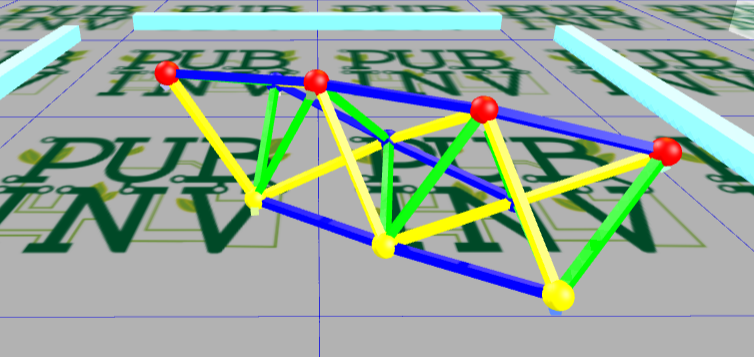
\includegraphics[width=0.4\textwidth]{figures/Tetrahelix1.png}
     \caption{2/3rd Twisted Tetrahelix}
     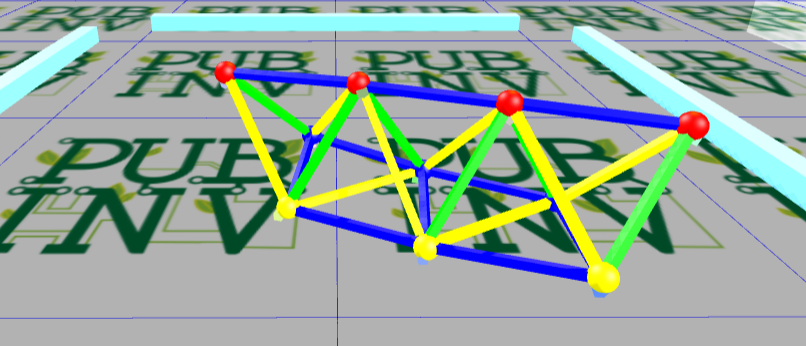
\includegraphics[width=0.4\textwidth]{figures/Tetrahelix2.png}
     \caption{1/3rd Twisted, 2/3rd Untwisted Tetrahelix}
     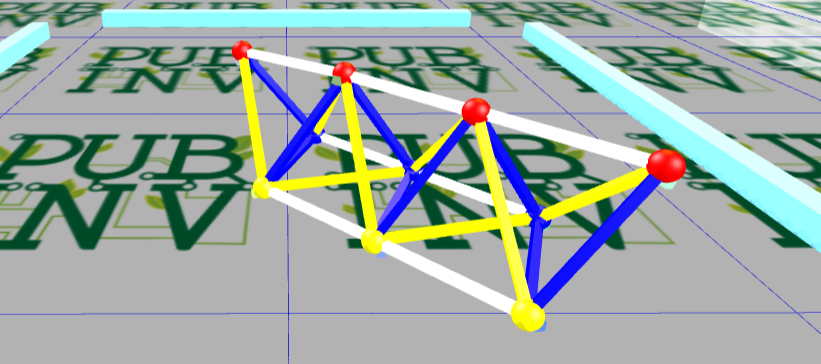
\includegraphics[width=0.4\textwidth]{figures/Tetrahelix3.png}
     \caption{The Equitetrabream: Fully Untwisted Tetrahelix}
\end{figure}

\section{Contact and Getting Involved}

The Gluss Project \url{http://pubinv.github.io/gluss/}
is a free-libre, open-source research, hardware, and software project that welcomes volunteers.
It is our goal to organize projects for the benefit of all humanity without seeking profit or intellectual property.
To assist, contact \href{mailto:read.robert@gmail.com}{$<$read.robert@gmail.com$>$}.

\bibliographystyle{IEEEtran}
\bibliography{IEEEabrv,gluss}

\end{document}

TODO:

Review and continue editing, being careful to introduce concepts in the correct order.

The most important thing to do here is to start a github project that includes javascript
to copute this stuff; the second most important thing is to use Three.js to create a
nice visual representation of all of this without getting the physics engine involved.

Check formula to make sure lengths are what we previously created for the Equitetrabeam.

First, plug values into Equitetrabeam.

Check distances.

Also, update diageam.



  Investigate Lambda outsidde the range [0,1].  Does -lambda reverse the chirality?
  Does lambda > 1 increase twist nicely?

  Create alternate coloring inside my system to render the tetrabot better.
  Add shadows better.

  Conjecture: There is a sense in which every tetrahelix has vertices
  evenly space along the axis of motion in order to have optimal lengths.

  Argument sketch: Follow current argument sketch, but compute lengths from formula
  for helices, using symmetry argument whereever possible.
  
  Create separate Github project having javascript code as function for computing all.

  Make YouTube video.

  
